GrandeOmega has been tested extensively with students from Hogeschool Rotterdam, a university of applied science in the Netherlands. The classes were divided into two groups: in the first classes were given some programming assignments to be completed in the traditional way (without GrandeOmega), while in the second other classes were asked to solve the assignments both in the traditional way and in GrandeOmega. Table \ref{tab:performance_go} and Figure \ref{fig:bar_chart} contain data relative to the pass rate and average grades of the classes that were asked to used also GrandeOmega, with and without using it. Table \ref{tab:prediction} and Figure \ref{fig:prediction} contain data relative to the accuracy of the prediction on the student success performed by GrandeOmega. The total number of students who participated is 241.

The data shows that the use of GrandeOmega enhanced the pass rate of classes 1B and 1C, but not that of 1F, 1L, and 1A. This means that the students of 1B and 1C failed questions in the traditional way that they were able to solve in GrandeOmega. Nonetheless, we can see that it always enhanced the grades of all the classes by at least 4\%. Moreover, if we compare the average passing grade of these classes with those who never used GrandeOmega, we can see that we reach a difference of even 12\%.

GrandeOmega was revealed to be effective even in predicting the success of students with a total reliability of 77\%, based on the percentage of assignment completed correctly.

\begin{table}[!h]
	\begin{tabular}{|p{0.1\columnwidth}|p{0.1\columnwidth}|p{0.1\columnwidth}|p{0.1\columnwidth}|p{0.1\columnwidth}|p{0.1\columnwidth}|}
		\hline
		\textbf{Class} & Completions & Pass rate & Pass rate G.O. & Average grade & Average grade G.O. \\
		\hline
		INF1B & 71.8 & 3 & 14 & 84.7 & 97.2 \\
		\hline
		INF1F & 56.7 & 6 & 5 & 77.0 & 88.1 \\
		\hline
		INF1L & 48.1 & 2 & 2 & 75 & 83.8 \\
		\hline
		INF1A & 41.7 & 7 & 7 & 82.1 & 86.5 \\
		\hline
		INF1C & 35.6 & 5 & 7 & 82.5 & 93.3 \\
		\hline
	\end{tabular}
	\caption{Student performance before and after GrandeOmega}
	\label{tab:performance_go}
\end{table}

\begin{table}[!h]
	\begin{tabular}{|p{0.2\textwidth}|p{0.2\textwidth}|p{0.2\textwidth}|p{0.2\textwidth}|p{0.2\textwidth}|}
		\hline
		\textbf{Class} & \textbf{Correct prediction} & \textbf{False positive} & \textbf{False negative} & \textbf{Incorrect prediction} \\
		\hline
		INF1B & 16 & 8 & 2 & 10 \\
		\hline
		INF1F & 11 & 2 & 4 & 6 \\
		\hline
		INF1L & 18 & 3 & 1 & 4 \\
		\hline
		INF1A & 13 & 0 & 2 & 2 \\
		\hline
		INF1C & 15 & 1 & 1 & 2 \\
		\hline
	\end{tabular}
	\caption{Prediction of student performance}
	\label{tab:prediction}
\end{table}

\begin{table}[!h]
	\begin{tabular}{|p{0.25\textwidth}|p{0.25\textwidth}|p{0.25\textwidth}|p{0.25\textwidth}|}
		\hline
		\textbf{Class} & \textbf{Average grade} & \textbf{Passed students} & \textbf{Avarage passing grade} \\
		\hline
		INF1H & 41.4 & 3 & 83.3 \\
		\hline
		INF1E & 30.6 & 1 & 75 \\
		\hline
		INF1J & 23.3 & 0 & N.A. \\
		\hline
		INF1G & 41.4 & 7 & 80.3 \\
		\hline
	\end{tabular}
	\caption{Results of classes without GrandeOmega}
	\label{tab:performance_no_go}
\end{table}

\begin{figure}[!h]
	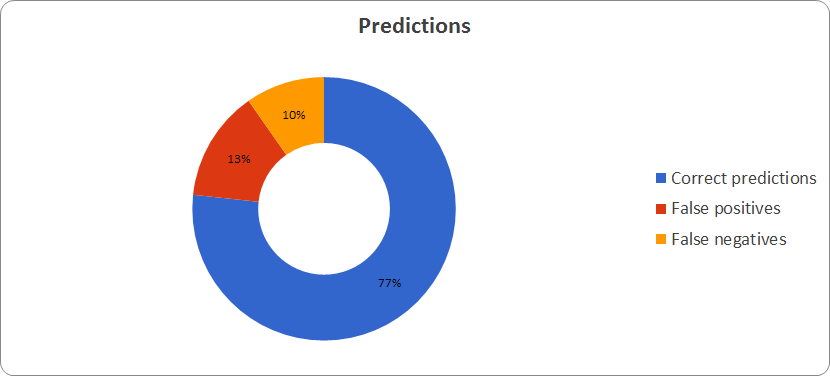
\includegraphics[width = \columnwidth]{Figures/prediction}
	\caption{Predition accuracy of GrandeOmega}
	\label{fig:prediction}
\end{figure}

\begin{figure}[!h]
	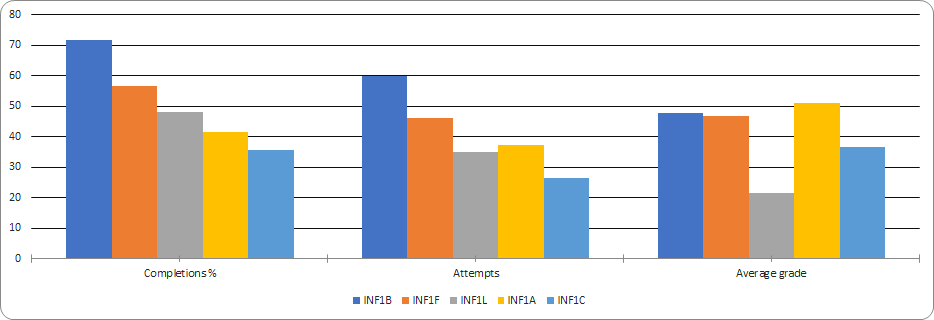
\includegraphics[width = \columnwidth]{Figures/bar_chart}
	\caption{Student performance with and without G.O.}
	\label{fig:bar_chart}
\end{figure}